\makeatletter
\def\input@path{{headers/}}
\makeatother
\documentclass{beamer}

\usepackage{beamer_tom}
\usepackage{hyperref}
\graphicspath{{./images/}{/home/tom/Pictures/People/}}


\institute{INRIA Saclay}
\author{Thomas Moreau}
\title{
    Benchopt:\\
    How standard is the performance of ResNet18 on CIFAR10?
}


\setbeamertemplate{title page}[frame]
\def\extraLogo{}


\begin{document}

    \begin{frame}
        \titlepage
    %	\biblio{}
    \end{frame}

    \frame{
        \frametitle{ResNet18 on CIFAR10}

        {\bf CIFAR10:} Image classification of $32\times32$ images from 10 classes.\\[2em]

        {\bf ResNet18:} \emph{de facto} baseline for this task for many developments:\\[.5em]
        \hskip1ex \myitem{} Optimizers,
        \hskip1ex \myitem{} Data Augmentation,
        \hskip1ex \myitem{} Architecture,
        \hskip1ex \myitem{} ...\\[2em]
        \strongpoint{However, replicating SOTA for this architecture\\is actually quite hard!}

        \vskip1em
        \keypoint{and many failed...}

        \vskip1em
        The goal of {\bf Benchopt} is to make this step as easy as possible.

    }

    \frame{
        \frametitle{Benchopt}

        \centering
        \vskip1.5em
        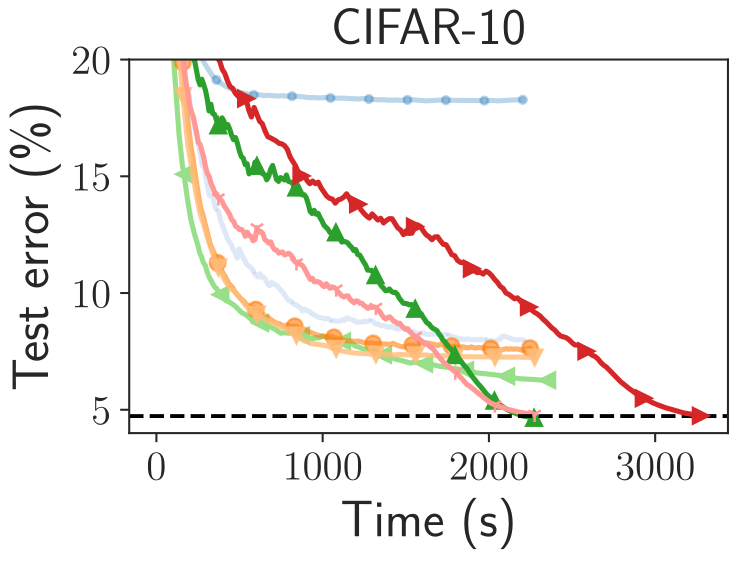
\includegraphics[width=.6\textwidth]{cifar10}\\
        \vskip2em
        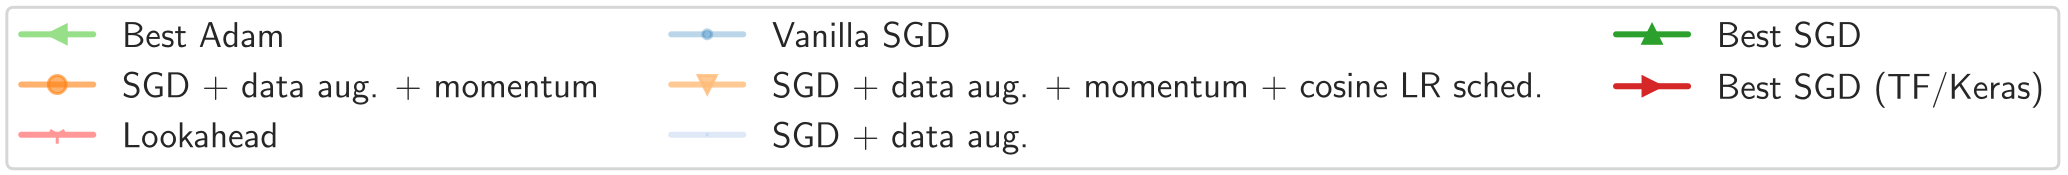
\includegraphics[width=\textwidth]{cifar10_legend}\\
    }

    \frame{
        \frametitle{Extra comparisons}

        \begin{itemize}\itemsep2em
            \item Multiple datasets: MNIST, SVHN, CIFAR10, CIFAR100, ...
            \item Matching \texttt{PyTorch} and \texttt{Tensorflow}.\\[.5em]
            {\centering
            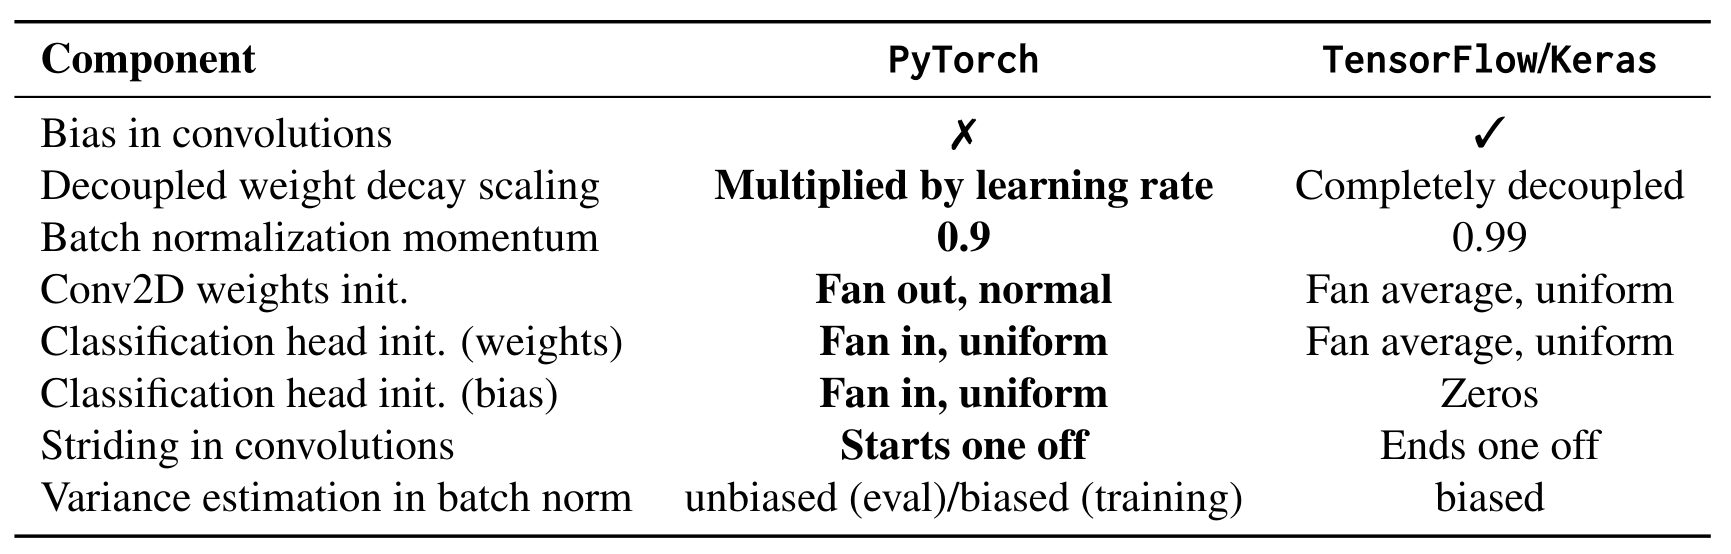
\includegraphics[width=.7\textwidth]{pytorch_tf.png}\\}
            \item Evaluated the impact of cross-validation,
        \end{itemize}

    }

    \frame{
        \frametitle{Benchmarks}
        You can run a similar benchmark with the correct baseline from:\\[1em]

        {\centering \url{https://github.com/benchopt/benchmark_resnet_classif}\\[2em]}

        Most of the heavy liftinghave been done together with:\\[2em]

        {\centering \hfill\includegraphics[width=.19\textwidth]{zramzi}\hfill
        \includegraphics[width=.19\textwidth]{pablin}\hfill\phantom{.}\\
        \hfill Zaccharie Ramzi\hfill
        Pierre Ablin\hfill\phantom{.}\\[2em]}

        Arxiv paper: \url{https://arxiv.org/abs/2206.13424}
    }

\end{document}